\documentclass[11pt]{report}

\usepackage{graphicx}

\begin{document}

\title{CS663 Assignment-5 Question-1 Report}
\author{KOTWAL ALANKAR SHASHIKANT | 12D070010}
\maketitle

The generated scatter-plot is shown below:\newline \newline
\centerline{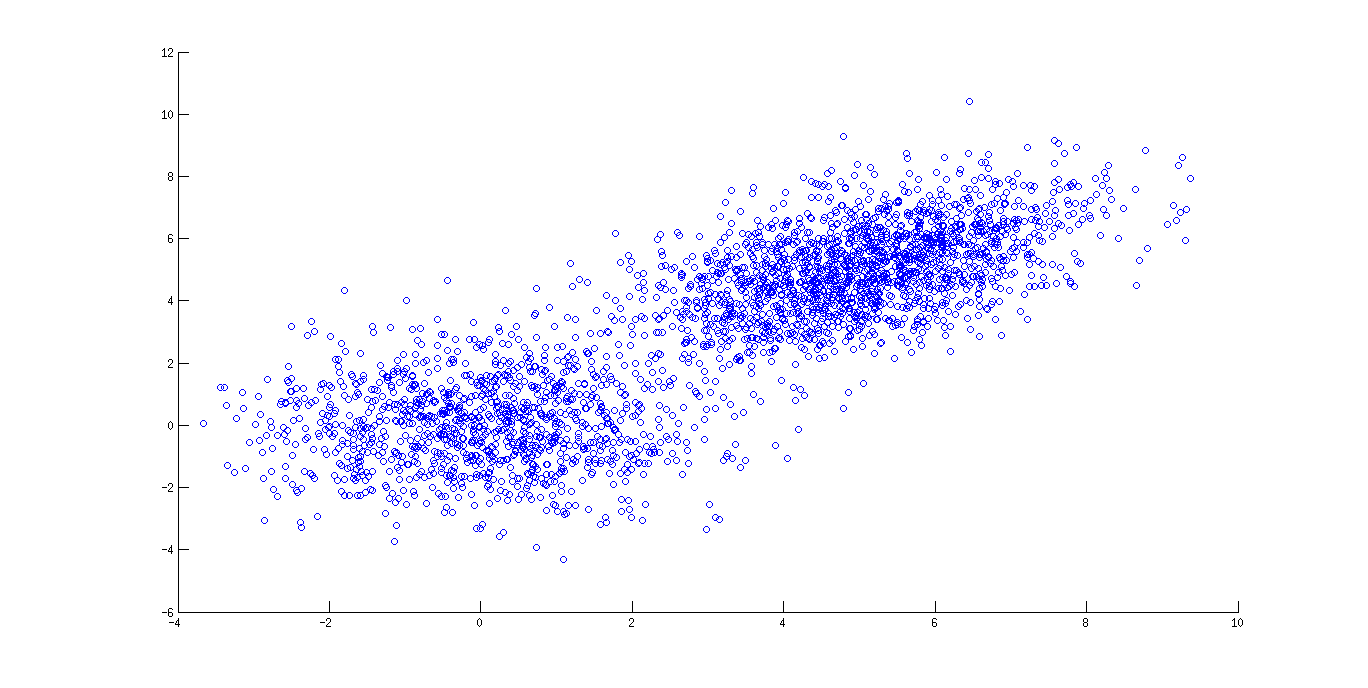
\includegraphics[scale=0.3]{scatter.png}}
\newline
\newline
Note that the blob centred at zero looks non-circular because scales of the axes are not the same.
\newline
After mean-shift, the new points are marked in green on the same plot:
\centerline{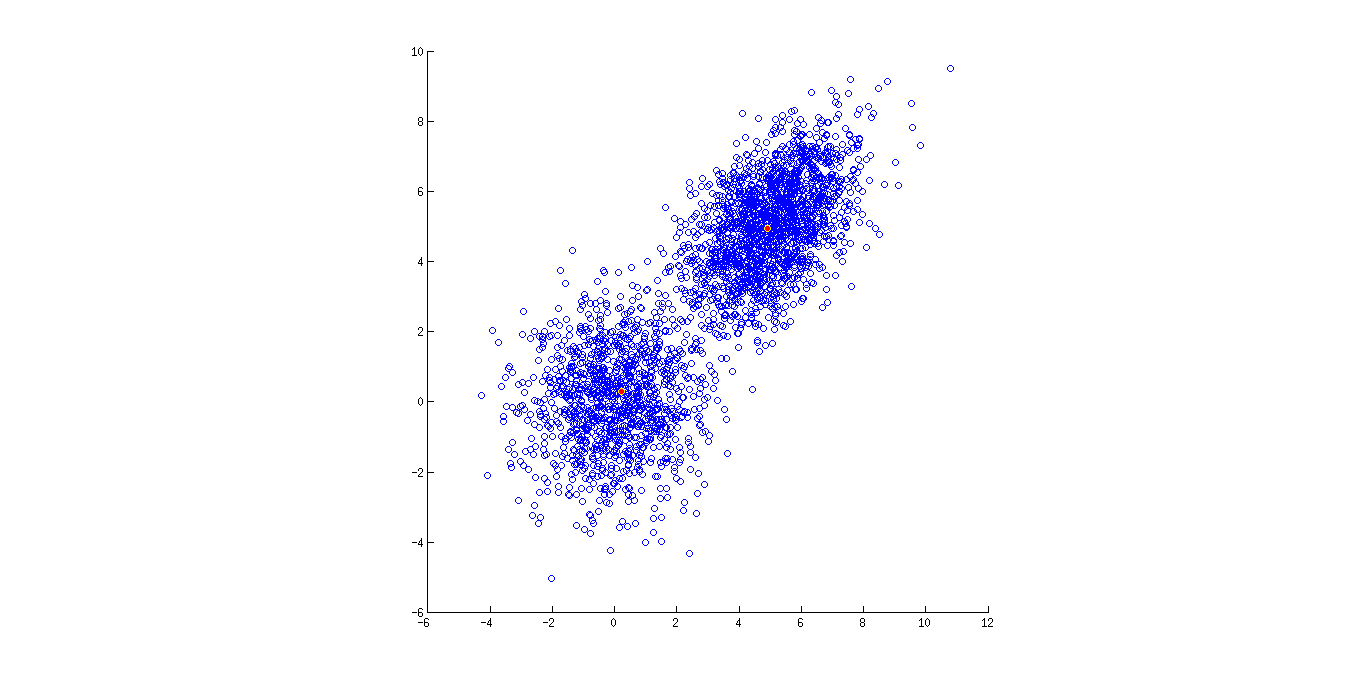
\includegraphics[scale=0.3]{cluster.png}}
\newline
\newline
For the 3000 sample points in the given distribution, and for a minimum movement of 0.0000001 between iterations, the minimum number of convergence steps is 2. The maximum is 5, and the average is 3.35.

\end{document}